Although \eko{} is totally \pdf{} independent, for the sake of plotting
we choose NNPDF4.0~\cite{NNPDF:2021njg} as a default choice for
our plots, but for \cref{sec:pheno:bench} where we choose the toy \pdf{} of the
Les Houches Benchmarks~\cite{Giele:2002hx,Dittmar:2005ed}.
We show the gluon distribution $g(x)$ as a
representative member of the singlet sector and the valence distribution $V(x)$
as a representative member of the non-singlet sector.
Note that \pdf{}s in the same sector have mostly the same behavior, apart from
some specific regions (e.g.\ the $T_{15}$ distribution right after charm
matching).

\subsection{Benchmarks}
\label{sec:pheno:bench}
In this section we present the outcome of the benchmarks between \eko{} and similar 
available tools assuming different theoretical settings.

\subsubsection{Les Houches Benchmarks}
\eko{} has been compared with the benchmark tables
given in \cite{Giele:2002hx,Dittmar:2005ed}.
We find a good match except for a list of typos which we list here:
\begin{itemize}
    \item in table head in \cite{Giele:2002hx} should be $2xL_+ = 2x(\bar u + \bar d)$
    \item in the head of table 1: the value for $\alpha_s$ in \ffns{} is wrong (as pointed out and corrected in \cite{Dittmar:2005ed})
    \item in table 3, part 3 of \cite{Giele:2002hx}: $xL_-(x=10^{-4}, \muF^2 = \SI{1e4}{\GeV^2})=1.0121\cdot 10^{-4}$ (wrong exponent) and
          $xL_-(x=0.1, \mu_F^2 = \SI{1e4}{\GeV^2})=9.8435\cdot 10^{-3}$ (wrong exponent)
    \item in table 15, part 1 of \cite{Dittmar:2005ed}: $xd_v(x=10^{-4}, \mu_F^2 = \SI{1e4}{\GeV^2}) = 1.0699\cdot 10^{-4}$ (wrong exponent) and
          $xg(x=10^{-4}, \mu_F^2 = \SI{1e4}{\GeV^2}) = 9.9694\cdot 10^{2}$ (wrong exponent)
\end{itemize}
Some of these typos have been already reported in \cite{Diehl:2021gvs}.

\begin{figure}
    \centering
    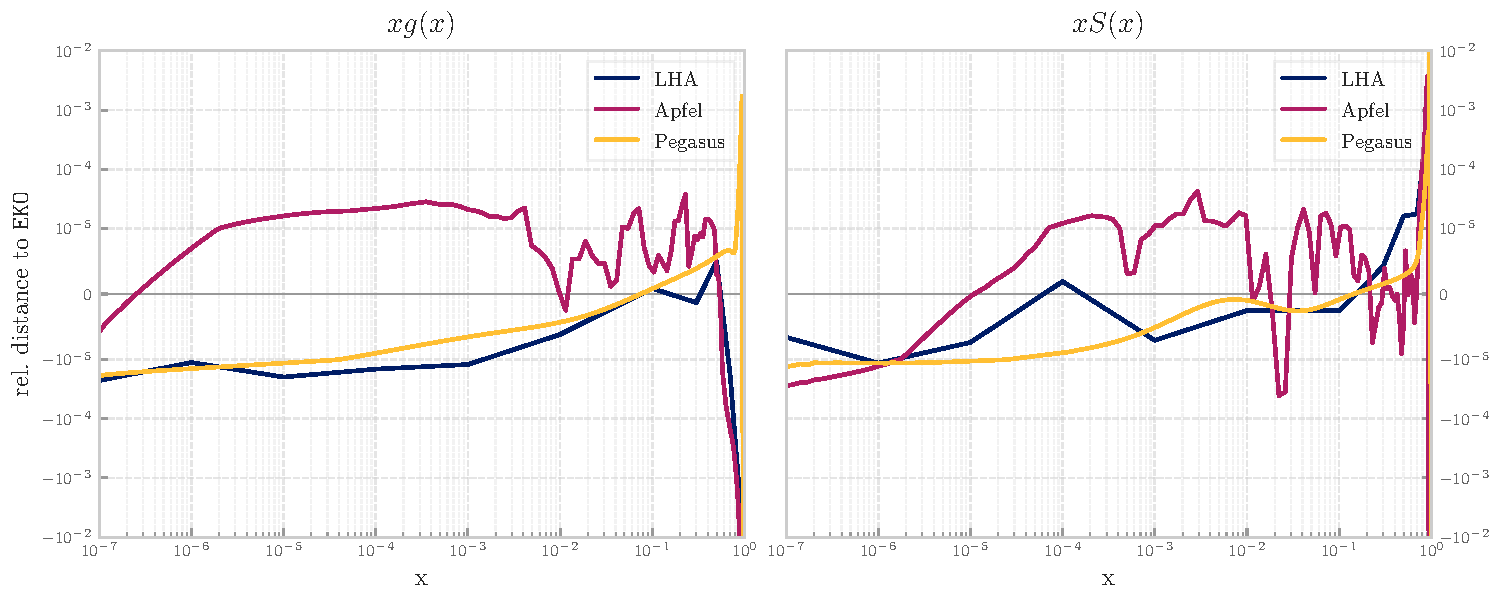
\includegraphics[width=\textwidth,height=.24\textheight]{ch-eko/lha_bench_g_S}
    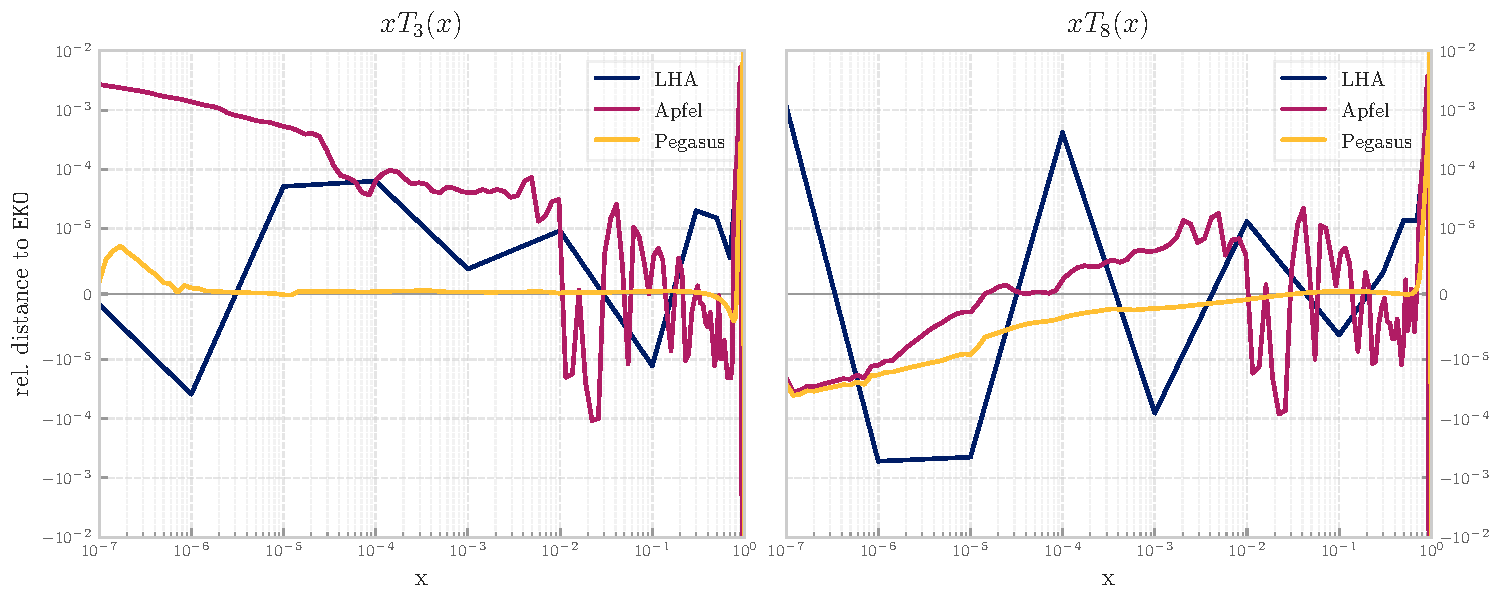
\includegraphics[width=\textwidth,height=.24\textheight]{ch-eko/lha_bench_T3_T8}
    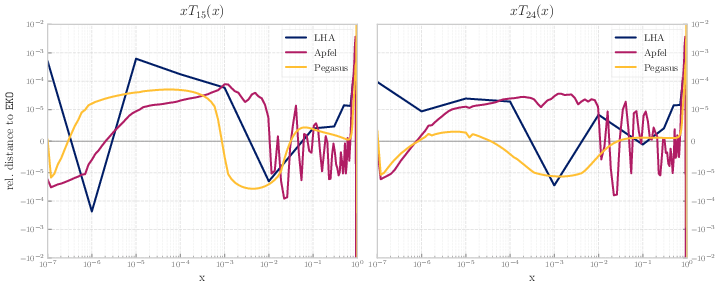
\includegraphics[width=\textwidth,height=.24\textheight]{ch-eko/lha_bench_T15_T24}
    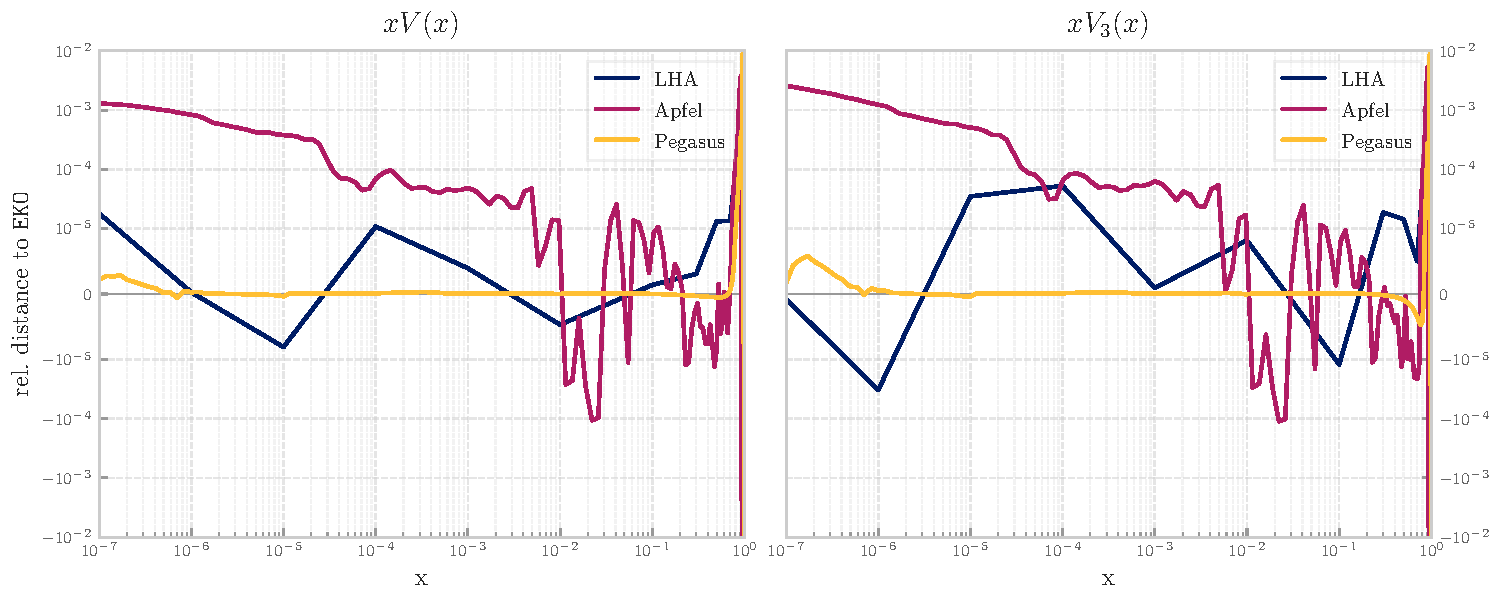
\includegraphics[width=\textwidth,height=.24\textheight]{ch-eko/lha_bench_V_V3}
    \caption{Relative differences between 
        the outcome of \nnlo{} \qcd{} evolution
        as implemented in \eko{} and the
        corresponding results from \cite{Dittmar:2005ed}, \apfel{}~\cite{Bertone:2013vaa} and \pegasus{}~\cite{Vogt:2004ns}.
        We adopt the settings of the Les Houches \pdf{} evolution benchmarks~\cite{Giele:2002hx,Dittmar:2005ed}.}
    \label{fig:LHAbench}
\end{figure}

In \cref{fig:LHAbench} we present the results of the \vfns{} benchmark at \nnlo{}, where a
toy \pdf{} is evolved from $\mu_{F,0}^2=\SI{2}{\GeV^2}$ up to $\mu_{F}^2=\SI{1e4}{\GeV^2}$
with equal values of the factorization and renormalization scales $\muF=\muR$.
For completeness, we display the singlet $S(x)$ and gluon $g(x)$ distribution (top), the singlet-like $T_{3,8,15,24}(x)$ (middle)
and the valence $V(x)$, valence-like $V_{3}(x)$ (bottom) along with
the results from \apfel{} and \pegasus{}. We find an overall agreement at the level of $O(10^{-3})$.


\subsubsection{APFEL}
\apfel{} \cite{Bertone:2013vaa} is one of the most extensive tool aimed to
\pdf{}  evolution and \dis{} observables calculation.
It is provided as a Fortran library, and it has been used by the NNPDF
collaboration up to NNPDF4.0~\cite{NNPDF:2021njg}.

\apfel{} solves \dglap{} numerically in $x$-space, sampling the evolution
kernels on a grid of points up to \nnlo{} in \qcd{}, with \qed{} evolution also
available at \lo{}.
By construction this method is \pdf{} dependent and the code is automatically
interfaced with \lhapdf{}~\cite{Buckley:2014ana}. For specific application,
the code offers also the possibility to retrieve the evolution operators
with a dedicated function.

The program supplies three different solution strategies, with various theory
setups, including scale variations and \msbar{} masses.

The stability of our benchmark at different perturbative orders is presented in \cref{fig:eko/Apfelbench_pto},
using the settings of the Les Houches \pdf{} evolution benchmarks~\cite{Giele:2002hx,Dittmar:2005ed}.
The accuracy of our comparison is not affected by the increasing complexity
of the calculation.

\begin{figure}
    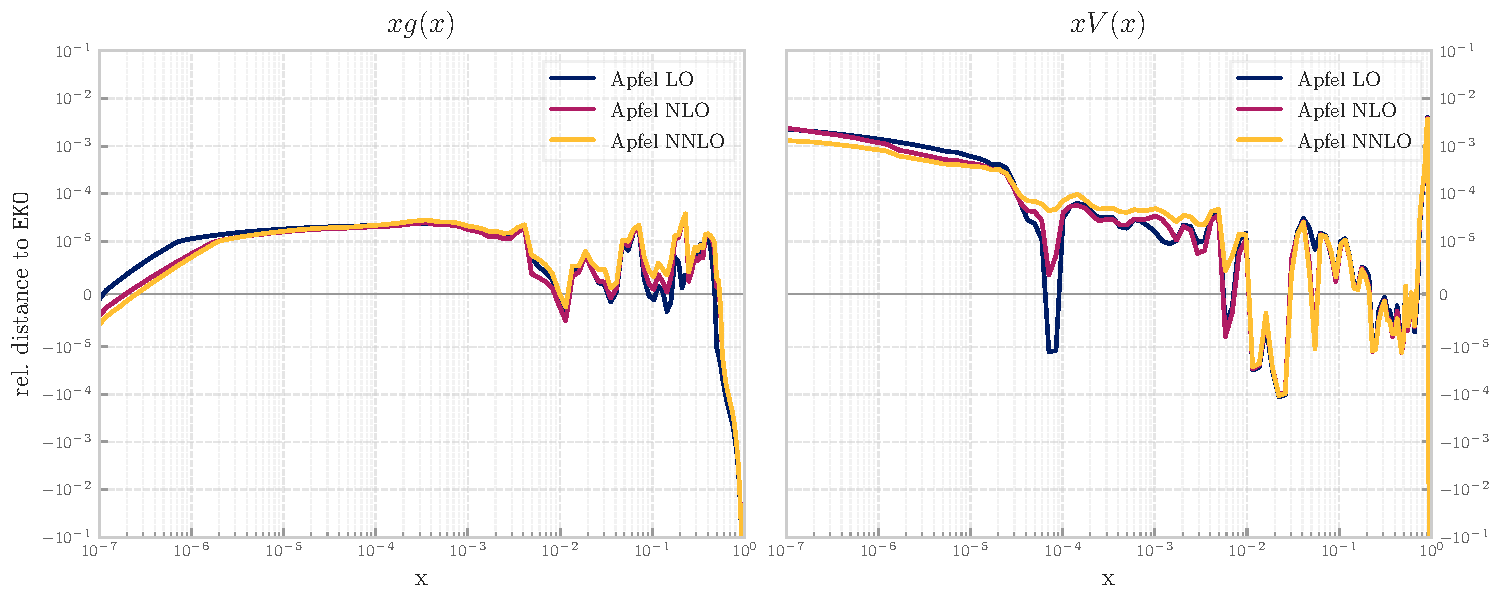
\includegraphics[width=\linewidth]{ch-eko/Apfel_bench_pto.pdf}
    \caption{Relative differences between the outcome of evolution as
        implemented in \eko{} and the corresponding results from \apfel{} at
        different perturbative orders.  We adopt the same settings of
        \cref{fig:eko/LHAbench}.}
    \label{fig:eko/Apfelbench_pto}
\end{figure}


\subsubsection{PEGASUS}
\pegasus{}~\cite{Vogt:2004ns} is a Fortran program aimed for \pdf{} evolution.
The program solves \dglap{} numerically in $N$-space up to \nnlo{}.
\pegasus{} can only deal with \pdfs given as a fixed functional form and is
not interfaced with \lhapdf{}.

As shown in \cref{fig:eko/LHAbench}, the agreement of \eko{} with this tool is better than with \apfel{},
especially for valence-like quantities, for which an exact solution is possible, where we reach
$\mathcal{O}(10^{-6})$ relative accuracy.
This is expected and can be traced back to the same \dglap{} solution strategy in Mellin space.

Similarly to the \apfel{} benchmark, we assert that the precision of our benchmark with \pegasus{} is not affected
by the different \qcd{} perturbative orders, as visible in \cref{fig:eko/Pegasusbench_pto}.
As both, \apfel{} and \pegasus{}, have been benchmarked against
\hoppet{}~\cite{Salam:2008qg} and \qcdnum{}~\cite{Botje:2010ay} we conclude
to agree also with these programs.

\begin{figure}
    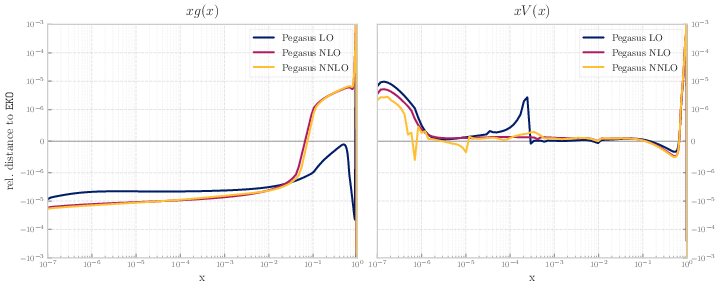
\includegraphics[width=\linewidth]{ch-eko/Pegasus_bench_pto.png}
    \caption{Same of \cref{fig:eko/Apfelbench_pto}, now comparing to \pegasus{}~\cite{Vogt:2004ns}.
        \label{fig:eko/Pegasusbench_pto} }
\end{figure}


%\subsubsection{Other tools}
%Finally we have benchmarked \eko{} comparing to other PDFs by means of \lhapdf{}.
In \cref{fig:eko/Hera_ct18_bench} we report a comparison of the evolution of
HERAPDF20 and CT18 at \nnlo{} from $\mu_{F}^2=\mu_{0}^2 \rightarrow 10^4~GeV$, where
$Q_{0}$ is the relative fitting scale.

During the fitting procedure two PDFs sets are evolved from the fitting scales
with different tools: respectively \hoppet{} and \qcdnum{}, while both collaborations used
\xfitter{} as a minimizer.

The benchmark with respect to HERAPDF20 indicates an agreement with \eko{}
both for singlet and valence-like quantities with a relative accuracy of $\mathcal{O}(10^{-3})$.
On the other hand the comparison with CT18 is more subtle and some discrepancies are visible
in the low-x region for valence-like quantities. We remark that even in this where the relative accuracy
deteriorate quickly, the absolute difference remains under control so the benchmark can be considered
acceptable.

\gmerror{Do we want to keep this benchmark?? Expand explanation ?}

\begin{figure}
      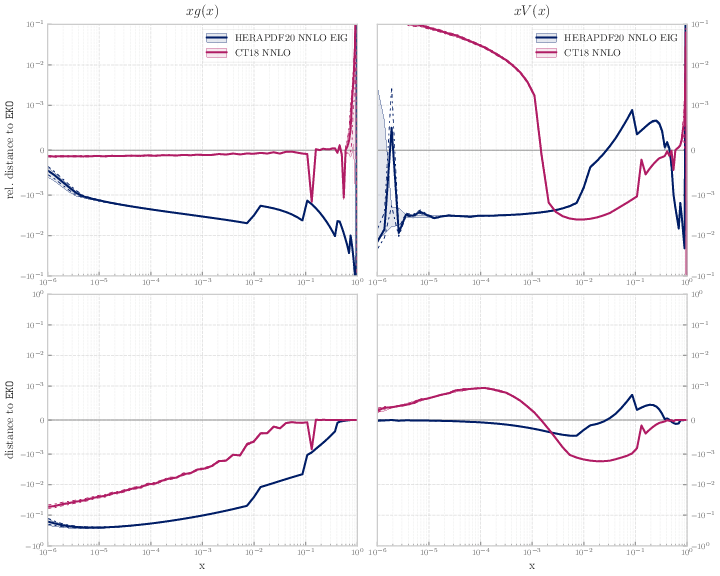
\includegraphics[width=\linewidth]{ch-eko/hera_ct18_bench.png}
      \caption{Relative (top)  and absolute (bottom) differences between
          the outcome of \nnlo{} \qcd{} evolution
          as implemented in \eko{} and the
          corresponding results from \lhapdf{} for HERAPDF20 and CT18.
          The evolution range is taken from the fitting scale to $\mu_{F}^2=10^4~GeV$.
          \label{fig:eko/Hera_ct18_bench} }
  \end{figure}



\subsection{Solution Strategies}
\label{sec:pheno:sols}
The formal solution of \cref{eq:eko/dglap2} in terms of evolution kernel
operators $\vb {\tilde E}$ is given by
\begin{equation}
    \vb {\tilde E}(a_s \leftarrow a_s^0)  = \Pd \exp\qty[-\int\limits_{a_s^0}^{a_s} \frac{\bm{\gamma}(a_s')}{\beta(a_s')} \dd{a_s'} ]
    \label{eq:eko/eko}
\end{equation}
with $\Pd$ the path-ordering operator. If the anomalous dimension $\bm{\gamma}$ is
diagonal in flavor space, i.e.\ it is in the non-singlet sector, it is always
possible to find an analytical solution to \cref{eq:eko/eko}. 
In the singlet sector sector, however, this is only true at LO and to obtain a
solution beyond, we need to apply different approximations and solution
strategies, on which \eko{} offers currently eight implementations. For an
actual comparison of selected strategies, cf.\ \cref{sec:eko/pheno-sols}.


\subsection{Interpolation}
\label{sec:pheno:interp}
To bridge between the desired $x$-space input/output and the internal
Mellin representation, we do a Lagrange-Interpolation as sketched in
\cref{sec:theory:interpolation}
(and detailed in the \href{https://eko.readthedocs.io/en/latest/}{online documentation}).
We recommend a grid of at least 50 points with
linear scaling in the large-$x$ region ($x \gtrapprox 0.1$) and with logarithmic
scaling in the small-$x$ region and an interpolation of degree four.
Also the grids determined by \amcfast~\cite{Bertone:2014zva} perform
sufficiently well for specific processes.

\begin{figure}
    \begin{center}
    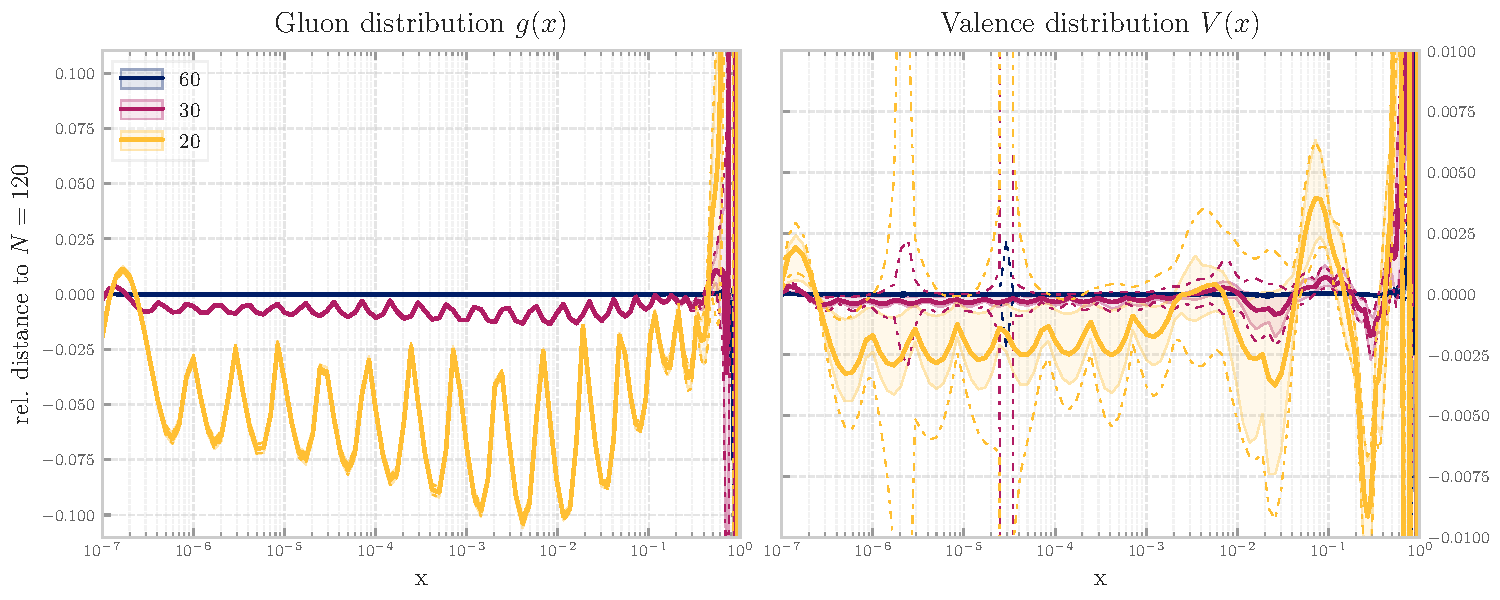
\includegraphics[width=\textwidth]{ch-eko/interpolation-int-ratio}
    \end{center}
    \caption{Relative differences between 
        the outcome of \nnlo{} \qcd{} evolution
        as implemented in \eko{} with 20, 30, and 60 points to 120
        interpolation points respectively.
        \label{fig:interpolation} }
\end{figure}

For a first qualitative study we show in \cref{fig:interpolation} a
comparison between an increasing number of interpolation points
distributed according to \cite[Eq. 2.12]{Carrazza_2020}.
The separate configurations are converging to the solution with the
largest number of points. Using 60 interpolation points is almost
indistinguishable from using 120 points (the reference configuration in the plot).
In the singlet sector (gluon) the convergence is
significantly slower due to the more involved solution strategies and,
specifically, the oscillating behavior is caused due to these difficulties.
The spikes for $x\to 1$ are not relevant since the \pdf{}s are intrinsically
small in this region ($\vb f\to 0$) and thus small numerical differences
are enhanced.

Also note that the results of \cref{sec:pheno:bench} (i.e.\ \cref{fig:LHAbench,fig:Apfelbench_pto,fig:Pegasusbench_pto}) confirm that
the interpolation error can be kept below the benchmark accuracy.


\subsection{Matching}
\label{sec:pheno:match}
\eko{} can perform calculation in a fixed flavor number scheme (\ffns{}) where
the number of active or light flavors $n_f$ is constant. This means that both
the beta function $\beta^{(n_f)}(a_s)$ and the anomalous dimension
$\bm{\gamma}^{(n_f)}(a_s)$ in \cref{eq:dglap2} are constant with respect to
$n_f$.
However, this approximation is likely to fail either in the high energy region
$\muF^2 \to \infty$ for a small number of active flavors, or to fail in the low
energy region $\muF^2 \to \Lambda_{\text{QCD}}^2$ for a large number of active
flavors.

This can be overcome by using a variable flavor number scheme (\vfns{}) that
changes the number of active flavors when the scale $\muF^2$ crosses a
threshold $\mu_h^2$.
This then requires a matching procedure when changing the number of active
flavors, and for the \pdf{}s we find
\begin{equation}
    \tilde{\mathbf{f}}^{(n_f+1)}(\mu_{F,1}^2)= \tilde{\mathbf{E}}^{(n_f+1)}(\mu_{F,1}^2\leftarrow \mu_{h}^2) {\mathbf{R}^{(n_f)}} \tilde{\mathbf{A}}^{(n_f)}(\mu_{h}^2) \tilde{\mathbf{E}}^{(n_f)}(\mu_{h}^2\leftarrow \mu_{F,0}^2) \tilde{\mathbf{f}}^{(n_f)}(\mu_{F,0}^2)
    \label{eq:matching}
\end{equation}
where the superscript refers to the number of active flavors and we split the matching into two
parts: the perturbative operator matrix elements (\ome{}) $\tilde{\mathbf{A}}^{(n_f)}(\mu_{h}^2)$,
currently implemented at \nnlo{}~\cite{Buza_1998}, and an algebraic rotation ${\mathbf{R}^{(n_f)}}$ acting
only in the flavor space $\Fd$.

For backward evolution this matching has to be applied in the reversed order.
The inversion of the basis rotation matrices $\mathbf{R}^{(n_f)}$ is simple,
whereas this is not true for the \ome{} $\mathbf{\tilde A}^{(n_f)}$ especially
in case of \nnlo{} or higher order evolution.
In \eko{} we have implemented two different strategies to perform the inverse
matching: the first one is a numerical inversion, where the OMEs are inverted
exactly in Mellin space, while in the second method, called \texttt{expanded},
the matching matrices are inverted through a perturbative expansion in $a_s$,
given by:
\begin{align}
    \qty(\mathbf{\tilde A}^{(n_f)})_{exp}^{-1}(\mu_{h}^2) &= \mathbf{I} - a_s(\mu_{h}^2) \mathbf{\tilde A}^{(n_f),(1)} + a_s^2(\mu_{h}^2) \qty[ \mathbf{\tilde A}^{(n_f),(2)} - \qty(\mathbf{\tilde A}^{(n_f),(1)})^2 ] + O(a_s^3)
    \label{eq:invmatchingexp}
\end{align}
with $\mathbf{I}$ the identity matrix in flavor space.


\subsection{Backward}
\label{sec:pheno:back}
As a consistency check we have performed a closure test verifying that after
applying two opposite \ekos{} to a custom initial condition
we are able to recover the initial \pdf{}. Specifically, the product of the
two kernels is an identity both in flavor and momentum space up to
the numerical precision. The results are shown in \cref{fig:eko/closure_test} in case of \nnlo{} evolution
crossing the bottom threshold scale $\mu_{F}=m_{b}$. The differences between
the two inversion methods are more visible for singlet-like quantities,
because of the non-commutativity of the matching matrix $\tilde{\mathbf{A}}_{S}^{(n_f)}$.  

\begin{figure}
    \begin{center}
    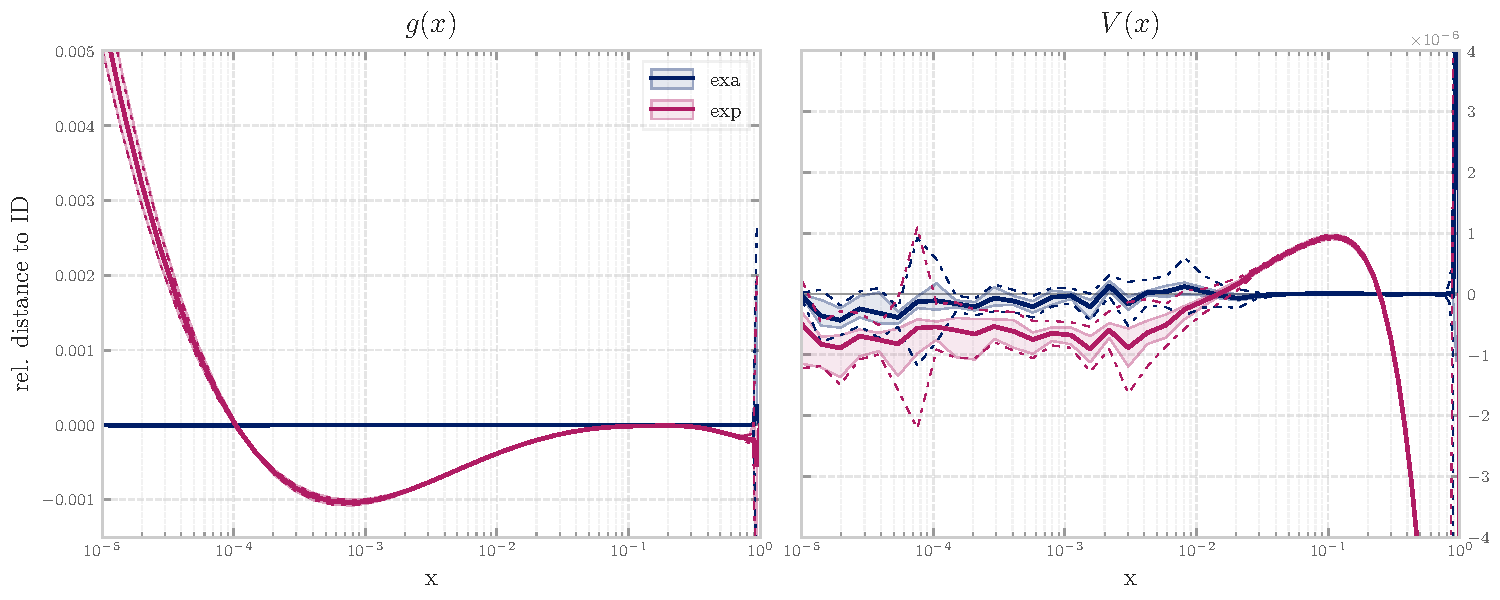
\includegraphics[width=\textwidth]{ch-eko/closure_test.pdf}
    \end{center}
    \caption{Relative distance of the product of two opposite \nnlo{} \ekos{}
        and the identity matrix, in case of exact inverse and expanded
        matching (cf.\ \cref{eq:eko/invmatchingexp}) when crossing the bottom
        threshold scale $\mu_{b}^2=\SI[parse-numbers=false]{4.92^2}{\GeV^2}$. In particular the lower scale is chosen $\muF^2=\SI[parse-numbers=false]{4.90^2}{\GeV^2}$, 
        while the upper is equal to $\muF^2=\SI[parse-numbers=false]{4.94^2}{\GeV^2}$, 
        \label{fig:eko/closure_test}
    }
\end{figure}

Special attention must be given to the heavy quark distributions which are
always treated as intrinsic, when performing backward evolution.
In fact, if the initial \pdf{} (above the mass threshold) contains an intrinsic contribution, this has to be evolved
below the threshold otherwise momentum sum rules can be violated.
This intrinsic component is then scale independent and fully decoupled
from the evolving (light) \pdfs.
On the other hand, if the initial \pdf{} is purely perturbative, it vanishes
naturally below the mass threshold scale after having applied the
inverse matching.
In this context, \eko{} has been used in a recent study to determine, for the first time,
the intrinsic charm content of the proton~\cite{Ball:2022qks}.


\subsection{\msbar{} masses}
\label{sec:pheno:msbarmass}
In \cref{fig:eko/MSbarbench} we investigate the effect of adopting a running mass
scheme onto the respective \pdf{} sets. The left panel shows the $T_{15}(x)$
distribution obtained from the NNPDF4.0 perturbative charm
determination~\cite{NNPDF:2021njg} using the pole mass scheme and the \msbar{}
scheme, respectively.
The distributions have been evolved on $\muF^2=\SI[parse-numbers=false]{1\to
10^4}{\GeV^2}$.
The mass reference values are taken from
\cite{LHCHiggsCrossSectionWorkingGroup:2016ypw}, with the \msbar{}
boundary condition on the charm mass given as $m_c(\mu_m=\SI{3}{\GeV}) =
\SI{0.986}{\GeV}$, leading to $m_c(m_c) = \SI{1.265}{\GeV}$, while the charm
pole mass is $m^\text{pole}_{c}\approxeq\SI{1.51}{\GeV}$~\cite{NNPDF:2021njg}.
The major differences are visible in the low-x region where the \dglap{}
evolution is faster and the differences between the charm mass treatment are
enhanced: an higher value of the charm mass increases the singlet like
distribution $T_{15}(x)$.
For the sake of comparison, in the right panel, we plot the relative distance
to our result when comparing with the \apfel{}~\cite{Bertone:2013vaa}
implementation.
As expected the pole mass results are closer due to the same value of the charm
mass, while the \msbar{} results have a slightly bigger discrepancy which
remains in all the $x$-range around $1\permil$ accuracy.

\begin{figure}
    \centering
    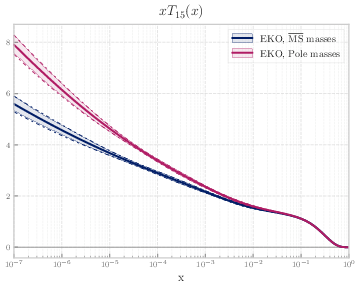
\includegraphics[width=0.47\linewidth]{ch-eko/msbar_T15.png}
    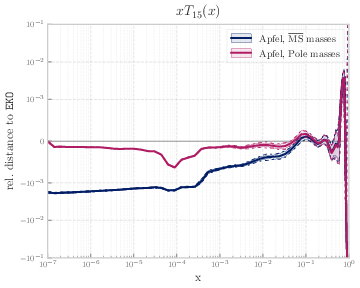
\includegraphics[width=0.47\linewidth]{ch-eko/msbar_bench_T15.png}
    \caption{(left) The NNPDF4.0 perturbative charm distribution
        $T_{15}(x)$~\cite{NNPDF:2021njg} with \msbar{} and pole masses \nnlo{}
        evolution when running on $\muF^2=\SI[parse-numbers=false]{1\to
        10^4}{\GeV^2}$.  (right) Relative difference to \eko{} for the same run
        with \apfel{}~\cite{Bertone:2013vaa}.}
     \label{fig:eko/MSbarbench}
\end{figure}

\begin{figure}
    \centering
    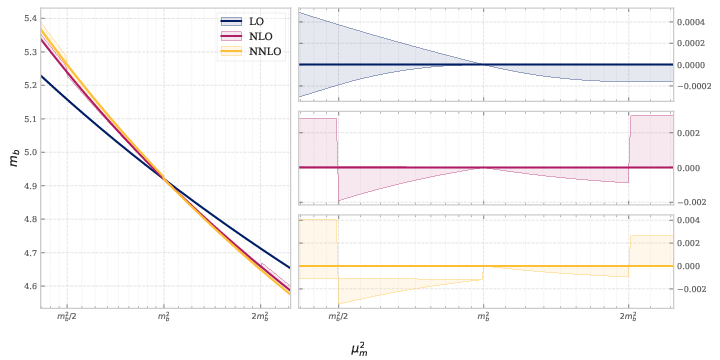
\includegraphics[width=\textwidth]{ch-eko/masses_running}
    \caption{Running of the bottom quark mass $m_b(\mu_m^2)$ for different threshold
        ratios, similar to \cref{fig:eko/asmatching}.
        The plot shows how the different choices of matching scales affect the
        running in the matching region (and slightly beyond) at \lo{}, \nlo{},
        and \nnlo{}.
        The border condition for the running has been chosen at $m_b(m_b) =
        \SI{4.92}{GeV}$, as it is clear from the plot, since it is the
        intersection point of all the curves shown.}
    \label{fig:eko/runningmasses}
\end{figure}


In \cref{fig:eko/runningmasses} we show the evolution of the \msbar{} bottom mass
$m_b(\mu_m^2)$ using different matching scales $\mu_b^2$ equal to $1/2,1$ and
$2$ times the mass $m_b^2$, for each perturbative order (\lo{}, \nlo{}, and
\nnlo{}).
The curve for $\mu_b^2 = m_b^2$ has been plotted as the central one (bold),
while the other two are used as the upper and lower borders of the shaded area
(according to their value, point by point).
The reference value $m_b(\mu_{b,0}^2)$, has been chosen equal for the
three curves, and it has been chosen at $m_b(m_b) = \SI{4.92}{GeV}$.
For this reason, above the central matching point $\mu_m^2 \ge m_b^2$ two curves coincide
($\mu_b^2 = m_b^2$ and $\mu_b^2 = m_b^2/2$) since they are both
running with the same number of flavors ($n_f=5$) and they have the same
border condition. The curve using $\mu_b^2 = 2m_b^2$, however, still runs with
a smaller number of flavors ($n_f=4$) and so does not match the former two.
In the lower region $\mu_m^2 < m_b^2$ this is not happening, because even
if the number of flavors is now the same,
the border condition is specified above matching for $\mu_b^2 = m_b^2$ (in
$n_f=5$).
So, starting from $m_b^2$ and going downward, the central choice $\mu_b^2 =
m_b^2$ is matched first and then evolved, while the higher scale choice
$\mu_b^2 = 2m_b^2$ immediately runs with four light flavors at $m_b^2$. Thus
the difference consists just in the matching.

